\chapter{Diseño del proyecto}\label{cap3}
Conforme a lo visto en el capítulo anterior, el proyecto requiere ser ejecutado de dos formas distintas (ejecución de automatizaciones y portal de usuario), además necesita de una base de datos para persistir los datos de las órdenes de reposición atendidas, catálogos y datos de usuario, también es necesario acceso al sistema de archivo para guardar las capturas de pantalla de las órdenes de reposición enviadas. Es decir, es requerido tener dos ambientes de ejecución, la automatización que será ejecutada exclusivamente en el sistema operativo y la de web, que si bien también estará contenida en el sistema operativo también es previsto que se ejecute parte del sistema en el explorador del usuario.


%===============================================================================
%===============================================================================


\section{Diseño de la arquitectura}
La definición estricta de arquitectura de software es:
\begin{center}
	``El conjunto de estructuras necesarias para la comprensión de un sistema en el cual se comprometen elementos de software, relaciones entre ellos y sus propiedades.''\cite{SWEBOOK}
\end{center}
En las últimas décadas la arquitectura de software ha profundizado en el estudio genérico de las estructuras del software, dando lugar a técnicas como Patrones de Diseño y Arquitectura 4+1.\\
\paragraph*{Patrones de Diseño}: ``Un patrón describe un problema recurrente sobre un ambiente, y entonces describe la técnica que soluciona el problema de forma tal que puede ser utilizado sobre cualquier instancia del problema.''\cite{DesignPatterns}. Esto quiere decir que dados los requerimientos funcionales del sistema es posible analizar la comunicación entre sus distintas partes y de esta forma saber lo patrones que son útiles para dar solución. Los patrones son organizados en tres categorías:
\begin{itemize}
	\item \textbf{Creacionales}: describen la forma en que las entidades (objetos si se utiliza el paradigma orientado a objetos) del sistema son creadas.
	\item \textbf{Estructurales}: describen la organización entre las entidades del sistema.
	\item \textbf{Comportamiento}: describen la comunicación entre entidades del sistema
\end{itemize}
\paragraph*{Arquitectura 4+1}: Organiza cada decisión en el diseño del sistema en cuatro partes llamadas vistas, cada vista se encarga de enfocarse en un aspecto del diseño, estas cuatro vistas son unificadas por una cuarta vista de escenarios o casos de uso (ver Figura \ref{fig:dia-arq-4-1}):
\begin{itemize}
	\item \textbf{Vista Lógica}: son las reglas del negocio por las que se rige la operación del usuario final.
	\item \textbf{Vista de Proceso}: refleja concurrencia y sincronización.
	\item \textbf{Vista de Física}: describe las relaciones del software con el hardware.
	\item \textbf{Vista de Desarrollo}: describe la organización estática del software en su ambiente de desarrollo.\cite{ViewModel4plus1}
\end{itemize}

\begin{figure}[h]
\centering
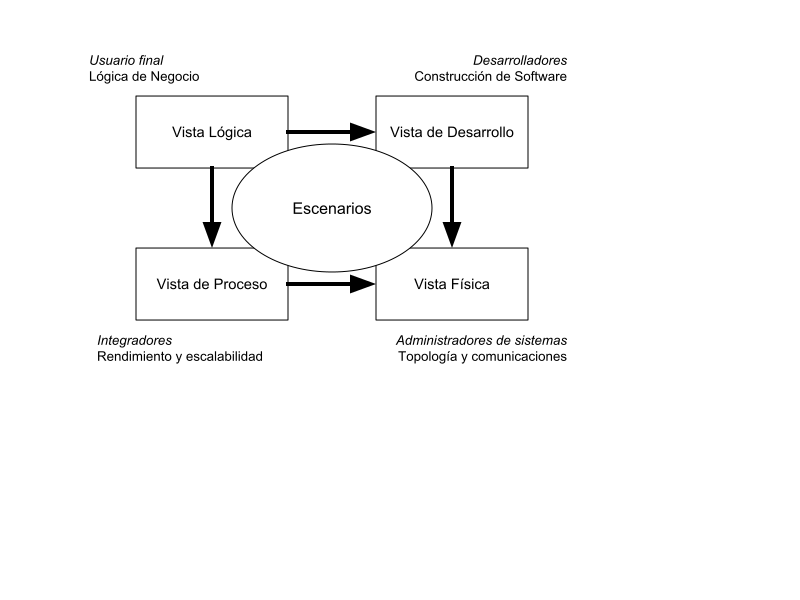
\includegraphics[width=\textwidth]{dia-arq-4-1} 
\caption{Diagrama de arquitectura 4+1.}
\label{fig:dia-arq-4-1}
\end{figure}

Tomando como referencia el modelo ``4+1'' descrito anteriormente, a esta altura se han presentado los escenarios, capítulo \ref{cap2}, y la vista lógica, capítulo \ref{cap1}, a continuación se tratarán temas que conciernen a la vista de Proceso y la vista Física, tocando un poco la vista de Desarrollo, pero esta última será explorada a profundidad en el siguiente capítulo.\\

\textcolor{red}{Esto sería una descripción breve del contenido de cada vista}
\textcolor{blue}{no estoy tan seguro... a ver que sale}

Vista de Desarrollo:
Vista de Proceso:
Vista Física:

\subsection{Componentes del sistema AutoSA}
El diagrama de componentes sirve para visualizar los componentes en los que se divide el sistema y las interfaces por las cuales se comunican tales componentes, el la Figura \ref{fig:dia-components} se muestra el diagrama de componentes para el sistema AutoSAI.
\begin{figure}[h]
\centering
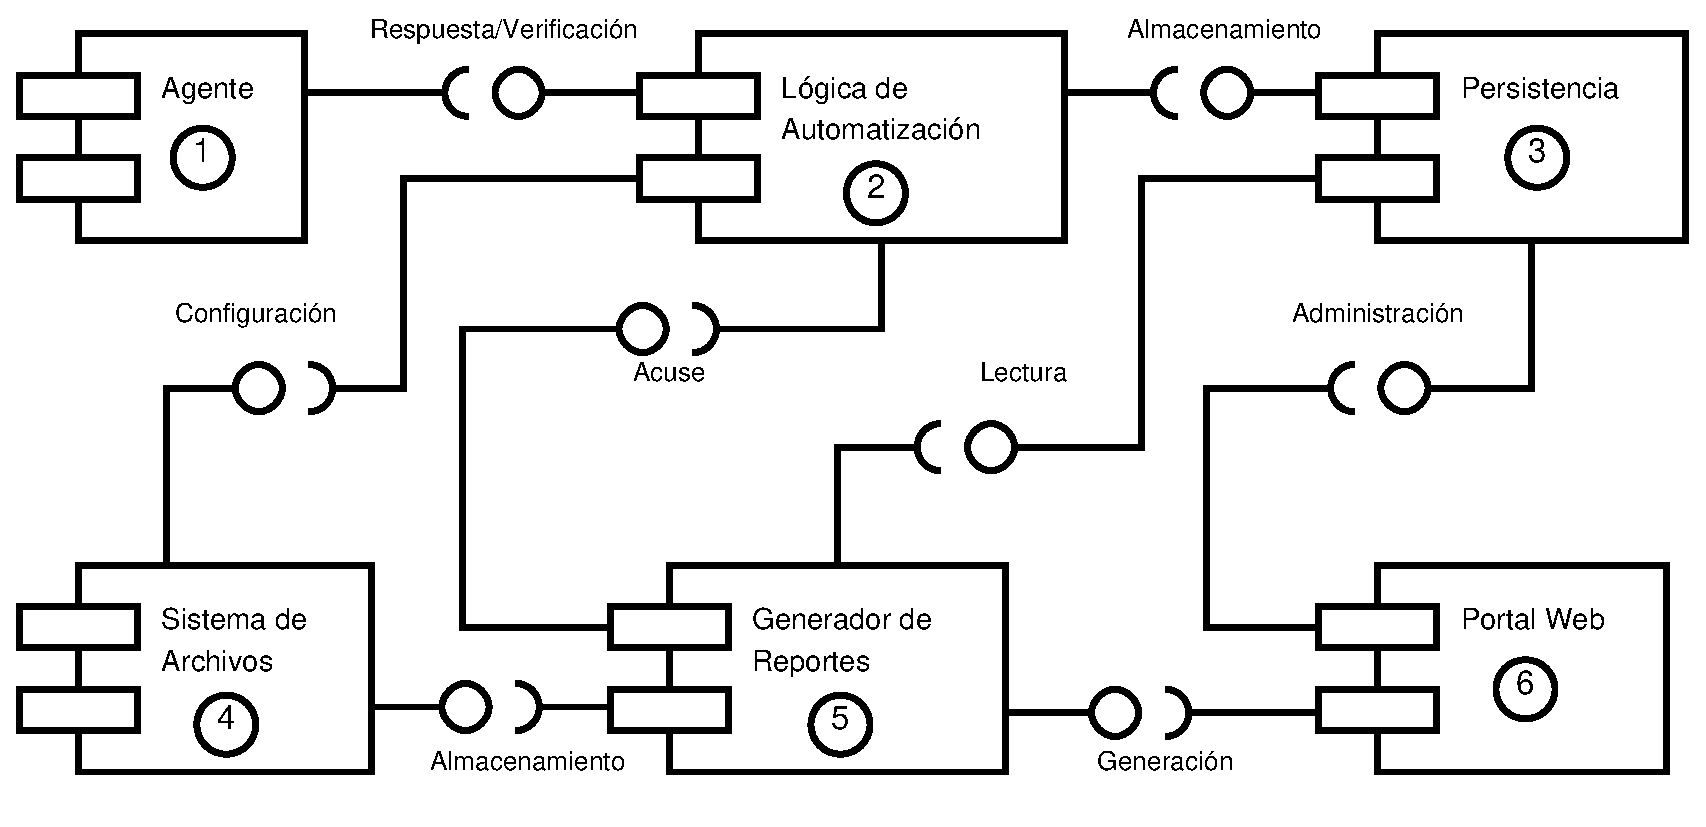
\includegraphics[width=\textwidth]{dia-components}
\caption{Diagrama de componentes.}
\label{fig:dia-components}
\end{figure}

A continuación se muestran las interfaces mediante las cuales los componentes ofrecen conjuntos de operaciones.

\subsubsection{Persistencia}
Este componente se encarga de la comunicación con la base de datos, es decir, realizar las acciones de guardar, modificar, borrar y buscar. 
\begin{enumerate}
\item \textbf{Almacenamiento} Da las operaciones necesarias parara crear y almacenar datos de órdenes de reposición en la base de datos.
\item \textbf{Lectura} Provee consultas a la base de datos para obtener reportes.
\item \textbf{Administración} Son las operaciones que permiten modificar datos específicos de las órdenes de reposición contenidas en la base de datos, también ofrece la actualización masiva de catálogos.
\end{enumerate}

\subsubsection{Sistema de archivos}
El componente Sistema de archivos es el único que se comunica con el sistema de archivos del sistema operativo\footnote{En este documento se utilizará de forma indistinta el término Sistema de archivos para referirse tanto al componente del sistema AutoSA como al propio del sistema operativo.}, tiene la función de realizar lectura de archivos de configuración, guardar los acuses de envío  y los reportes de las ordenes de reposición.
\begin{enumerate}
\item \textbf{Configuración} Da la configuración contenida en archivos de propiedades contenidas en el mismo sistema de archivos.
\item \textbf{Almacenamiento} Almacena los reportes y acuses de envío.
\end{enumerate}

\subsubsection{Lógica de automatización}

\begin{enumerate}
\item \textbf{Respuesta} Provee el acceso a las reglas de negocio del proceso de respuesta de órdenes de reposición.
\item \textbf{Verificación} Provee el acceso a las reglas de negocio del proceso de verificación de órdenes de reposición canceladas.
\end{enumerate}


\subsubsection{Generador de reportes}
El generador de reportes, como su nombre lo indica, tiene la función de generar documentos y reportes con los datos de las órdenes de reposición almacenados en la base de datos. 
\begin{enumerate}
\item \textbf{Acuse} Genera el documento con el acuse de envío.
\item \textbf{Generación} Genera reportes con los datos de las órdenes de reposición almacenados en la base de datos.
\end{enumerate}

\subsubsection{Robot}
El componente que contiene y ejecuta las rutinas de automatización. 

\subsubsection{Portal Web}
Es componente que ofrece al usuario las funcionalidades de una interfaz web. 


%===============================================================================
%===============================================================================
%
%
%\section{Diseño de la base de datos}
%La base de datos tiene dos finalidades, guardar la información capturada de las órdenes de reposición atendidas así como los catálogos necesarios para los procesos automatizados y generación de reportes; la segunda es guardar la información de los usuarios autorizados para utilizar el portal web.\\
%Tablas para automatización:
%\begin{itemize}
%	\item Órdenes de reposición: contiene la información capturada de las órdenes de reposición atendidas
%	\item Catálogo de estados de atención: estados por lo que pasa una orden de reposición cuando es atendida, tal y como se mostró en el diagrama <<hacer cita al diagrama de estados>>.
%	\item Catálogo de estados SAP: contiene los estados que puede tener una orden de reposición que ya ha sido contestada, es decir, vigente y cancelada.
%	\item Catálogos con claves de medicamentos y centros de salud.
%	\item Tablas para contener usuario del portal web:
%	\item Información de usuario: 
%	\item Credenciales de usuario
%\end{itemize}
%
%
%===============================================================================
%===============================================================================
%
%
%\section{Diseño de bibliotecas}
%
%
%===============================================================================
%===============================================================================
%
%
%\section{Diseño de rutinas de automatización}
%
%
%===============================================================================
%===============================================================================
%
%
%\section{Diseño de servicios}
%\subsection{Persistencia}
%\subsection{Acceso y Autorización}
%\subsection{Ordenes de Reposición}
%\subsection{Reportes}
%
%
%===============================================================================
%===============================================================================
%
%
%\section{Diseño de interfaz de usuario}
%
%

